\documentclass[a4paper, 10pt, american, titlepage]{article}

% useful packages
\usepackage[utf8]{inputenc} % UTF-8 support
\usepackage{minted} % for code snippets
\usepackage[american]{babel} % for changing particular titles
\usepackage{csquotes} % recommended for biblatex
\usepackage{graphicx} % for images
\usepackage[gen]{eurosym} % for literally just the euro symbol
\usepackage{lipsum} % lorem-ipsum placeholder text
\usepackage{bookmark} % links to other parts of the PDF
% if we want to use a different style, here are some to look at
% https://www.overleaf.com/learn/latex/Biblatex_bibliography_styles
\usepackage[backend=biber,style=numeric,sorting=none]{biblatex} % citations
\usepackage[page, titletoc, title]{appendix} % labeled appendices
\usepackage[margin=1in]{geometry} % set 1in margins
\usepackage{hyperref} % hyperlinks
\usepackage{setspace} % setting custom spacing
\usepackage{tabulary} % nicer tables
\usepackage{CJKutf8} % for Japanese UTF-8 characters

% more breathing room
\setminted{fontsize=\small,baselinestretch=1}

% correct bad hyphenation here
\hyphenation{op-tical net-works semi-conduc-tor}

% stuff for LaTeX to know
\bibliography{references}
\graphicspath{ {./images/} } % put images in here
\title{%
	\huge ARuko and Editour: \\
	\Large A Platform for Augmented Reality Tour Guide Apps}
\author{William~Campbell, Cole~Granof, and Joseph~Petitti}
\date{October 11, 2019}

% uncomment this to call it "Table of Contents" instead of just "Contents"
% \addto{\captionsamerican}{\renewcommand*{\contentsname}{Table of Contents}}

% custom environment for indenting whole paragraphs
\newenvironment{indented}[1]%
{\begin{list}{}%
	{\setlength{\leftmargin}{#1}}%
	\item[]%
}
{\end{list}}

\begin{document}

% set page numbers to Roman for the forematter (before the introduction)
\pagenumbering{roman}

% draw the title page
\maketitle

% more breathing room
\setstretch{1.5}

\begin{abstract}
	% abstract goes here
	\begin{figure}[h]
		\centering
		\includegraphics[width=\textwidth]{abstract.jpg}
		% Note: you don't actually need the part in square brackets for the
		% caption, but if you omit it the regular caption text will be used for
		% the List of Figures entry.
		\caption[\textit{Number 1, 1950 (Lavender Mist)}, Jackson Pollock]
		{\textit{Number 1, 1950 (Lavender Mist)}, Jackson Pollock, National
			Gallery of Art, Washington, D.C.}
		\label{fig:abstract}
	\end{figure}
\end{abstract}

\section*{Acknowledgments}
\label{sec:acknowledgements}
\addcontentsline{toc}{section}{Acknowledgments}

We would like to thank Atticus Sims, CEO and founder of Kyoto VR, for sponsoring
this project and providing help and guidance throughout our time in Japan. His
knowledge of the history of Kinkaku-ji and Kyoto in general has been invaluable
to our experience.

We would also like to thank Inoue Hikaru for his help with translations and
researching AR technology. A special thank you to the IQP team working with
Kyoto VR, Lewis Cook, Nicole Escobar, Ahad Fareed, and Cameron Person, for
filming and editing the app trailer, as well as providing help with testing.

Finally, a thank you to our advisers, Professors Joshua Cuneo and Ralph Sutter.
Without their expert advice and feedback this project probably could not have
been completed.

\clearpage

\section*{Executive Summary}
\label{sec:executiveSummary}
\addcontentsline{toc}{section}{Executive Summary}

Our team built, tested and polished a mobile app to deliver an audio tour,
incorporating various augmented reality (AR) features to enhance the
experience. Our app delivers a tour of Kinkaku-ji, or The Temple of the Golden
Pavilion, a popular tourist destination in Kyoto. In this app, which we call
ARuko, many of the AR features were aimed at improving accessibility. These
features include translating signs and providing additional info on the
physical map located at the site. Other features were purely for spectacle,
such as the ability to take an AR ``souvenir'' home by scanning the ticket
to enter Kinkaku-ji.

ARuko went through multiple iterations of user testing and bug testing at
Kinkaku-ji. Sections \ref{sec:initialFieldTesting} and
\ref{sec:finalFieldTesting} go into detail about our two days of field testing
on-site. From these tests, we were able to refine the user experience, and
identify important features to add to the app. Much of the app's functionality
was dictated by Atticus Sims, C.E.O and founder of Kyoto VR, who plans to
monetize the app. We also worked with an IQP team, who had been tasked with
exploring funding options and creating promotional content.

Since our app had to deliver an audio tour supplemented by images based on your
latitude and longitude, we developed an internal tool to design physical
regions for each step of the tour. This tool, called Editour provides a rich
editing suite through a simple web interface. Section~\ref{sec:editingATour}
goes into detail about the features of this web app. We also wrote a backend to
manage the tour files, allowing one of us (or our sponsor, Atticus Sims) to
download a zip file containing all of the media and info to reconstruct the
tour. This zip can be extracted into the source files for ARuko, which rebuilds
the tour from the downloaded contents. We were able to host the backend on the
server provided by Kyoto VR's hosting plan; we discuss the hurdles that we
overcame to deploy the Editour backend with Kyoto VR's current setup in
Section~\ref{sec:deployingTheEditourBackend}.

In Section~\ref{sec:alternativeArAppConcepts}, we also discuss the alternative
AR app concepts that were explored before development became completely focused
on ARuko.

\clearpage

% now comes the table of contents, list of figures, and list of tables
% these should be single spaced
\begin{singlespace}
	\tableofcontents
	% uncomment this if you want the Table of Contents to have an entry in the
	% table of contents
	% \addcontentsline{toc}{section}{Table of Contents}
	\clearpage

	\listoffigures
	% \addcontentsline{toc}{section}{List of Figures}
	\clearpage

	\listoftables
	% \addcontentsline{toc}{section}{List of Tables}
	\clearpage
\end{singlespace}

% go back to 1.5 spacing and Arabic numbering for the rest of the paper
\pagenumbering{arabic}

\section{Introduction}
\label{sec:introduction}

The field of consumer-oriented augmented reality (AR) technology is just coming
into full swing, and it presents many unique opportunities for a myriad of
fields. This budding technological platform uses digital displays to augment
real-world information with computer-generated data. As the technology
progresses, several disparate industries have found novel uses for it, some
becoming extremely profitable~\autocite{webster2018}. With smartphone
manufacturers investing billions into AR technology~\autocite{mason2016}, it
seems poised to be the next big digital interface.

Tourism and art are among the fields that could gain the most from AR
technology~\autocite{saenz2009, katz2018}. This technology can provide
accessible information to tourists and art viewers that they would not be able
to get any other way. Kinkaku-ji, the ``Golden Pavilion'' of Kyoto, is the
perfect example of a site that would benefit from AR~\autocite{bornoff2000}.
Kinkaku-ji is a UNESCO World Heritage Site~\autocite{unesco} and one of the
most popular tourist destinations in Japan~\autocite{japanguide2019}. The
Golden Pavilion is a magnificent sight to behold, but the gardens and grounds
are the true beauty of Kinkaku-ji. It is a living masterpiece of Zen Buddhist
landscape design, expanding on the natural beauty of Kyoto's forests and
mountains through the practice of borrowed scenery~\autocite{kuitert2002}.

However, much of the historic information at the site is lost on visitors
because it is not readily available to non-Japanese speakers. What few signs and
displays exist are presented only in Japanese, and do not provide most of the
history and context necessary to fully understand Kinkaku-ji.

To solve this problem and open up the peerless beauty of the Golden Pavilion to
more people, our team created ARuko and Editour. These two tools comprise a
complete platform for designing and experiencing AR-enhanced tours. Editour
makes it easy to design custom audio tours including audio, text, and images,
while ARuko allows users to seamlessly experience historic sites in an intuitive
and novel way. The experience of walking through the site is enhanced by
informative narration and AR pop-ups that do not alter the buildings or ground
in real life.

\clearpage

\section{Background}
\label{sec:background}

As smartphones and mobile technology become more prevalent, new forms of
human-computer interaction are becoming mainstream. Smartphones allow for an
unprecedented degree of connectivity with the digital world, but can also serve
as a tool for enhancing the physical world. In this section we explain the
origins and uses of some of this technology.

\subsection{What is Augmented Reality?}
\label{sec:whatIsAugmentedReality}

Augmented reality, or AR, is a type of human-computer interface where
perceptions of the real world are enhanced by computer-generated information.
This differs from virtual reality (VR) in that a VR experience consists
exclusively of virtual information. In AR, virtual information is mixed with
sensory input from the real world~\autocite{carmigniani2011}. This can enhance
the user's perception of reality by providing information that would be
difficult or impossible to display through traditional means.

For example, AR can be used to display information about historical events,
places, and objects overlaid onto images of the real
world~\autocite{saenz2009}.  This provides the user with useful information
without needing to alter a real historic site.

\subsubsection{Current Augmented Reality Technology}
\label{sec:currentAugmentedRealityTechnology}

While preparing for this project our team researched the current state of AR
technology. Smartphones are the most commonly used AR hardware by
far~\autocite{boland2018}. Typically smartphone AR applications make use of the
phone's camera, accelerometer, gyroscope, and GPS sensors to reproduce a view
of the real world with virtual information layered on top of
it~\autocite{bonsor2018}.

\subsubsection{Augmented Reality Use Cases}
\label{sec:augmentedRealityUseCases}

Even though it is still a developing technology, AR has been used in many
disparate disciplines, including data visualization~\autocite{resnick2017},
commerce~\autocite{matney2018}, marketing~\autocite{sharma2015},
education~\autocite{stewart-smith2012}, visual art~\autocite{katz2018}, and
even archaeology~\autocite{eve2012}.

The video game industry has readily embraced augmented reality, leading to the
development of many AR games for smartphones and dedicated head-mounted
displays. Perhaps the most popular AR game, \textit{Pokémon Go}, has been
downloaded over a billion times~\autocite{webster2018}. This game makes use of
GPS and camera data to overlay game objects (in this case fictional monsters) on
top of images of the real world~\autocite{concepcion2016} (see Figure
\ref{fig:pokemonGo}).

\begin{figure}[h]
	\centering
	\includegraphics[width=.5\textwidth]{pokemon-go.jpg}
	\caption[A screenshot from the AR game \textit{Pokémon Go}]{A screenshot
		from the AR game \textit{Pokémon Go}~\autocite{vastateparks2016}.}
	\label{fig:pokemonGo}
\end{figure}

\subsubsection{Challenges of Augmented Reality}
\label{sec:challengesOfAugmentedReality}

Many of the existing applications using AR, in our eyes, do not leverage the
full potential of this emerging technology. As with any new field, our
understanding of AR and how to develop for it is limited. All sorts of
different challenges and limitations face the development and production of AR
apps. Here are some that we considered when working on our app.

Many of the applications and use cases that exist for AR right now are, simply
put, not very good. Many AR apps and features available on smartphones offer
very little in the way of functionality or practicality; quite simply, they are
primarily used for minor spectacles and simple
tricks~\autocite{theappsolutions2018}. For example, one of the most popular
apps to use AR, \textit{Pokémon Go}, primarily uses its AR feature to place a
Pokémon on top of a camera's video feed. Disappointingly, it does not interact
with anything around it. It just floats a fixed distance away from the user.

Additionally, in many cases where AR is used, the task could be accomplished as
well or better without AR~\autocite{theappsolutions2018}. Returning to the
\textit{Pokémon Go} example, when the AR feature is left on while capturing a
Pokémon, the extra power needed for this feature drains the device's battery
faster. Also, it makes it harder to hit the Pokémon with a Pokéball due to the
model drifting in the environment. On top of all of this, the performance of
the app suffers drastically, especially on older devices. All of these problems
detract from the ability to play and enjoy the game.

One of the major problems facing AR development as a whole---including our
project---is limited hardware. For starters, smartphone cameras present a
major limitation. Many smartphone cameras only capture images in 2D, which can
make generating AR content in a 3D world difficult without the use of QR or
barcode markers~\autocite{geospatialworld2018}. Additionally, GPS sensors on
smartphones can also be too imprecise for good AR
tracking~\autocite{geospatialworld2018}.

AR apps are most commonly designed for smartphones due to their relatively low
cost and how accessible they are. However, smartphones come with a host of
hardware limitations that make achieving satisfying AR capabilities difficult.
Additionally, AR apps for smartphones tend not to be very user-friendly, and
oftentimes even complicate the task or activity they were meant to
enhance~\autocite{theappsolutions2018}.  The alternative then is to turn to
dedicated hardware, like Microsoft's HoloLens. The issue is that dedicated
hardware like the HoloLens is very inaccessible and expensive; Microsoft only
offers developer editions of the HoloLens, and for the incredibly steep price
of \$3,500~\autocite{microsoft2019}.

The challenges we faced during development mirrored those that plague the
industry as a whole very accurately. We struggled with how exactly we would use
AR for our app in a way that benefited the experience as a whole. Despite our
initial apprehension, we believe the way we have integrated AR into our app
enhances the user experience. Hardware issues were definitely our biggest
challenge. Only one member of our team had a phone new enough to run AR technology at a
decent level, making testing of our application difficult.

\subsection{izi.TRAVEL}
\label{sec:iziTravel}

Before our project started, Kyoto VR was already using an app to deliver audio
tours. The app, called izi.TRAVEL, allows users to create audio tours with
audio and image files tied to specific locations in the real
world~\autocite{izitravel2015} (see Figure \ref{fig:iziTravel}). The app is
aimed at museums and city tours~\autocite{izitravel} but can be used for tours
of historic sites too.  Kyoto VR used the platform to make a simple audio tour
of Kinkaku-ji.

\begin{figure}[h]
	\centering
	\includegraphics[width=.5\textwidth]{izi-travel.png}
	\caption{A screenshot of the izi.TRAVEL app interface}
	\label{fig:iziTravel}
\end{figure}

\begin{figure}[h]
	\centering
	\includegraphics[width=\textwidth]{kinkakuji.jpg}
	\caption[The Golden Pavilion of Kinkaku-ji, Kyoto, Japan]{The Golden
		Pavilion of Kinkaku-ji, Kyoto, Japan~\autocite{davidson2005}}
	\label{fig:kinkakuji}
\end{figure}

Our group aimed to implement all the functionality of izi.TRAVEL and more in
our own app. See Section \ref{sec:aruko} for more details.

\subsection{Augmented Reality Platforms}
\label{sec:platforms}

Before we could start working on creating our app, we first needed to decide
which AR development platform to use. Based on our preliminary research, we
learned there are many powerful platforms available. There were many things we
needed to consider before deciding on a platform. These considerations included
what features the platform offered, which devices and operating systems the app
could run on, and the cost. Detailed below are some of the different platforms
we considered.

\subsubsection{ARCore and ARKit}
\label{sec:ARCoreAndARKit}

ARKit and ARCore are both frameworks that enable apps to take advantage of
powerful AR related features. ARKit is developed by Apple and can only be used
by iPhones~\autocite{summerson2018}. Google's ARCore framework can deploy to both
Android and iPhone. Many cross platform solutions will leverage the full
potential of their target platform by using either ARKit or ARCore ``under the
hood.'' Both ViroReact and Vuforia use ARKit or ARCore depending on the target
platform \autocites{vuforiaFusion}{moon2018}.

ARKit 3 aims to support a wide array of new features and will be available in
iOS 13~\autocite{apple2019}. Notably, one of these features is ``people
occlusion,'' which will allow virtual objects to be realistically obscured when
someone walks in front of the object. This kind of technology could be useful
for us since our app uses AR in crowded places.  As of August 2019, this
feature is not on the horizon for ARCore.

Both ARKit and ARCore have well-supported APIs for Unity. ARKit 3 support is
coming soon to Unity, along with all of the advanced features that it
brings~\autocite{stinson2019}.

\subsubsection{Wikitude}
\label{sec:wikitude}

Wikitude is another major AR development kit that is very prevalent in the
world of AR development. It has over 130,000 registered AR developers, and is
powering over 30,000 AR apps across smartphones, tablets, and smart
glasses~\autocite{wikitude2018}. It is easy to understand why Wikitude has so
many registered developers considering the list of features the platform
offers. Some of the features that appealed most to us were their ``Instant
Tracking,'' allowing for augmentation using flat surfaces; ``Image Tracking,''
allowing for augmentation using one or multiple 2D images; and ``Geo AR,''
allowing for creation of geo-markers at specific locations to trigger AR
content.

Wikitude supports Android, Apple, and Windows phones and tablets, as well as
smart glasses like the Epson Moverio, Microsoft HoloLens, and Vuzix smart
glasses. Additionally, many different development frameworks are capable of
running Wikitude's software development kit (SDK). According to Wikitude's
website, their SDK works with Windows, Android, and iOS development frameworks,
as well as ARCore and ARKit, Flutter, Cordova, Xamarin, and even Unity.

Based on this information, Wikitude was initially appealing to us. However, the
cost was a major issue. Wikitude is free for eligible startups, but given the
criteria they list on their site, we were not confident that we would qualify.
Aside from this option, Wikitude offers a 30-day demo license for \euro{499},
which was far beyond the resources available to us. They also charge
\euro{1990} for their SDK Pro, and \euro{2490} for their SDK Pro 3D. Given
these prices, and our very limited budget, we decided to consider other
options.

\subsubsection{motive.io}
\label{sec:motive.io}

The company motive.io previously was developing a product that would allow
users to create an engaging AR experience in the style of
\textit{Pokémon~Go}~\autocite{odom2017}. Their service would have purportedly
handled technical details such as hosting, storage, and user accounts. The
promotional video shows the creation of a location-based AR game where the user
pretends to hack into ATMs using the real-world locations of ATMs in a city.

Unfortunately, it appears that the company has completely pivoted off of this
idea, and has since moved to developing AR training
software~\autocite{motiveio}. We reached out to motive.io via email for any
advice they might be willing to give us, but we received no response.

\subsubsection{ViroAR}
\label{sec:viroAR}

Viro AR comes in two flavors: ViroReact and ViroCore\autocite{facebook2019}.
ViroCore allows developers to build an AR Application with Java. The
disadvantage of this is that ViroCore only allows developers to target Android,
which unfortunately made ViroCore not an option for our project. ViroReact is
the cross-platform option for ViroAR. ViroReact leverages the cross-platform
capabilities of React, which is Facebook's JavaScript Library for developing
user interfaces~\autocite{facebook2019}.

Since our project is not a game, we initially wanted to avoid using a
fully-featured game engine such as Unity (see Section~\ref{sec:unity}.
Therefore, we decided to take the time to explore this framework since it
appeared to be more tailored to our specific use case. Viro Media also
recognizes that all developers who wish to create an app with 3D capabilities
are not necessarily game developers. Viro Media pitches ViroAR as ``The
perfect alternative to specialized game engines, ViroAR is a platform for
rapidly building ARKit and ARCore apps. Our platform allows developers to focus
on what they do best by leveraging familiar tools and frameworks used in mobile
application development''~\autocite{viro2019}. While the majority of our team
has decent experience with writing JavaScript, we have have very little experience
writing React apps.

In most app development scenarios, to test the app on actual hardware, it must
be compiled using either Xcode or Android Studio depending on your platform.
Once you have built the app, your device needs to install the app. This process
can be very time consuming, especially when needing to run frequent tests on
the target platform.

An alternative to building an app for a physical phone is to run it through an
emulator on a computer.

According to Techopedia, ``Emulation is the process of imitating a
hardware/software program/platform on another program or platform. This makes
it possible to run programs on systems not designed for
them''~\autocite{techopedia2019}. Emulators are often very useful for speeding
up development. Loading programs onto the Android emulator is usually much
faster than installing an Android package file (APK) onto the actual device.
Additionally, emulators can mock almost all of the important features of an
actual Android device, including calls, text, GPS position, device rotation and
more~\autocite{androidemulator}.

Since an emulator uses software to emulate hardware, this poses two technical
issues that prevent emulators from being a proper replacement for testing on
real hardware. Emulation is often imperfect, so glitches sometimes emerge in
emulation that do not manifest on the actual hardware~\autocite{alzaylaee2017}.
Conversely, errors that exist in the hardware version may not appear in the
emulation. Secondly, and most importantly for AR, it is common for emulation to
be much slower compared to real hardware.

In a question submitted to \textit{Compute!} magazine asking whether it is
possible for a Commodore 64 to emulate MS-DOS, the editor responded ``Yes, it's
possible for a 64 to emulate an IBM PC, in the same sense that it's possible to
bail out Lake Michigan with a teaspoon.'' The editor goes on to explain
``Emulation is a complex business, but here's one rule of thumb: The only way
to successfully emulate a machine is with a much more powerful
machine''~\autocite{warick1988}. In our case, emulating Android on a desktop
operating system is closer to emulating a C64 on an IBM PC running MS-DOS
(rather than the other way around, thankfully). The takeaway is that the speed
problem facing emulators is just as real as it was in 1988. Considering that AR
already pushes modern phone hardware to the limit, emulation is not something
is not something we wanted to struggle with. On top of this, our testing
required us to move the camera through the world at various speeds and angles,
which is simply cumbersome with a laptop webcam.

As an alternative to emulation, ViroReact offers a convenient ``test bed'' for
rapidly testing your ViroReact app on native hardware without the need for an
emulator. In the root directory of your project, you can launch a Node server
with the command \texttt{npm start}. From here, you can input the provided URL
into the Viro Media app. This will quickly download the code, graphics, and 3D
object files from the server and launch a functional version of the app
\autocite{viro-testbed2019}. This allowed us to get a real AR app up and
running on our devices much more easily than any of the other
frameworks/engines we explored. Unfortunately, the test bed app was somewhat
unreliable based on our experience; the test bed would frequently crash or
would not be able to download the files from the Node server. The most reliable
way to test our app was to compile a binary and manually install it onto our
devices, which completely defeats the purpose of the test bed app.

\subsubsection{Unity}
\label{sec:unity}

\subsection{Kinkaku-ji}
\label{sec:kinkaku-ji}

Kinkaku-ji, the Temple of the Golden Pavilion, is undoubtedly one of Japan's
greatest attractions.  As of September 2019, it was the second-most visited site
in Kyoto---second only to Kyoto Station \autocite{japanguide2019}. Kinkaku-ji's
rich history and stunning beauty bring tourists from all over the world to see
its shining gold walls and magnificent gardens. Our project intends to enhance
user's enjoyment and understanding of Kinkaku-ji through informative interactive
media, teaching about the history and significance of the site.

The site that is now Kinkaku-ji was originally a villa owned by poet and
nobleman Saionji Kintsune, until the land was bought by shōgun Ashikaga
Yoshimitsu in 1397~\autocite{noboru2013}. As Zen Buddhism was in vogue among the
warrior class in Japan at the time, the site was converted into a Zen temple
according to Yoshimitsu's wishes upon his death~\autocite{bornoff2000}.

The main pavilion is a three-story tall building on the edge of a landscaped
pond. The outer walls of the top two floors are completely covered in gold leaf,
leading to the name ``Golden Pavilion'' (\begin{CJK}{UTF8}{min}金閣\end{CJK}
\textit{kinkaku}). The grounds surrounding the Golden Pavilion are in the style
of a Japanese strolling garden, with carefully manicured plants and paths and
designated viewing points. The buildings and landscaping make use of a Zen
practice called ``borrowed scenery'' (\begin{CJK}{UTF8}{min}借景\end{CJK}
\textit{shakkei}), in which the background landscape is incorporated into the
design of a garden~\autocite{noboru2013}.

The pavilion sits on the edge of a carefully designed pond (see Figure
\ref{fig:kinkakujiGrounds}), with small islands designed to replicate the shape
of Japan and several other famous locations from Japanese and Chinese
literature~\autocite{young2007}. All of these landscape features have been
immaculately maintained and preserved through the Golden Pavilion's six hundred
year history.

\begin{figure}[h]
	\centering
	\includegraphics[width=\textwidth]{kinkakuji-grounds.jpg}
    \caption[Expertly landscaped islands in the Kinkaku-ji mirror pond]{Expertly
		landscaped islands in the Kinkaku-ji mirror pond~\autocite{desousa2014}}
	\label{fig:kinkakujiGrounds}
\end{figure}

In 1950 the pavilion was burned down by a paranoid schizophrenic monk who had
been living at the temple~\autocite{borowitz2005}. The structure was rebuilt in
1955, close to the original design but with more extensive gold
leaf~\autocite{bornoff2000}. The interior was also restored later.

None of this history is readily apparent to a casual tourist at Kinkaku-ji.
There are a few signs describing different areas, but they are only available in
Japanese and contain very little information about the history and design of the
site. Because of this, an intuitive audio tour app with AR features would be
very helpful to tourists at Kinkaku-ji.

\clearpage

\section{Implementation and Technology}
\label{sec:implementationAndTechnology}

In this section we discuss and implementation of ARuko and Editour, including
the technologies and techniques involved in creating both of them. We also
discuss the design decisions we made and some of the challenges we faced in
creating these applications.

\subsection{Editour: The Tour Editor}
\label{sec:editour}

The goal of Editour is to allow a non-technical user to design audio tours
through a web-app. At its core, Editour is a tool to draw arbitrarily-shaped
geographic regions onto a map, edit those regions and assign media to each of
the drawn regions.

An audio file and multiple image files can be uploaded for each region the user
defines. The user can also provide a text transcript of the audio file as well.
After naming and uploading the tour with the ``Upload'' button, our backend
builds a zip containing a folder that can be placed directly into the Unity
project.

Our backend allows users to save their tours to our server and load those same
tours back into the editor to resume work.  The geographic area of each region
can be adjusted by clicking and dragging. Vertices can also be added and
deleted if the needs of the tour change over time.

\subsubsection{The Need for an Editor}
\label{sec:theNeedForAnEditor}

One of the goals for our project is to create a working prototype that others
can build off of in the future.

Similar to the app izi.TRAVEL discussed in Section~\ref{sec:iziTravel}, we
needed some way to easily define arbitrary polygons (which we call ``regions'')
and associate media with each one, such as audio and image files.

For testing purposes, we initially defined these regions directly in the C\#
Scripts, hard-coding the coordinates. Below is an example of a quadrilateral
surrounding the Creation Core building at the Ritsumeikan Biwako-Kusatsu campus.

\begin{minted}{csharp}
Regions.add(new GPSPolygon(new List<GPSPoint>{
    new GPSPoint(34.979222, 135.963628),
    new GPSPoint(34.979187, 135.965130),
    new GPSPoint(34.979794, 135.965053),
    new GPSPoint(34.979754, 135.963669)
}, "Creation Core"));
\end{minted}

Even with knowledge of C\# and Unity, inputting tour data this way is obviously
not convenient. Atticus reminded us that, although he has a working knowledge of
Unity, he is not a software developer. In order to make our app prototype at all
useful for the future, we needed to provide an easy way to ``design'' a tour.

\subsubsection{A Complete Tour Definition}
\label{sec:tourDefinition}

In order to create a fully-functional editor for designing and exporting
``tours,'' we had to consider how to fully define a tour purely in terms
of text and a directory of associated media.

Here is an example of the JSON metadata generated by Editour:

\begin{minted}{json}
{
   "regions": [
      {
         "name": "Beautiful Place",
         "points": [ {"lat": 34.979222, "lng": 135.963628}, ... ],
         "audio": [ "beautiful-audio.mp3" ],
         "images": [ "mountain.jpg", "stream.jpg" ],
         "transcript": "To your left, you can see a beautiful place."
      },
      {
         "name": "Gorgeous Place",
         "points": [ {"lat": 34.979754, "lng": 135.964889}, ... ],
         "audio": [ "gorgeous-audio.mp3" ],
         "images": [ "hill.jpg", "valley.jpg", "gorge.jpg" ],
         "transcript", "To your right, you can see a gorgeous place."
      }
   ]
}
\end{minted}

Within each object in the region list, we can see that the region has five
properties: a name, a list of coordinates, a list of audio files, a list of
multiple image files, and a transcript of the audio file. (In the current
design of the app, it only makes sense to associate one audio file per region,
but the format makes it easy to accommodate for multiple audio files in the
future.) One disadvantage is that all media files have to have unique names.
This is because the zip that is created by the Editour backend contains all of
the media files in a flat file structure. The above JSON is used to associate
each media file with a region, meaning that the filename needs to act as a
primary key. The backend will respond with a message if this is the case,
prompting the user to have unique names for all files.

\subsubsection{Editing a Tour}
\label{sec:editingATour}

The user can easily create a new region by shift-clicking, and then clicking
points on the map.  To terminate the polygon, the user must shift-click again.
The ``Welcome to Editour'' card (seen in Figure~\ref{fig:welcomeCard}) provides
these instructions, which should be enough to get started.  A user can only
terminate the polygon after two points have been placed to prevent the user
from drawing a region with an area of zero. Once a region is created, a region
card appears in the side bar. From here, the user can edit anything about the
region. From here, the user can edit anything about the region.

\begin{figure}[h]
	\centering
	\includegraphics[width=0.4\textwidth]{welcome-card-editour.png}
    \caption{The ``Welcome to Editour'' card providing basic instructions to
    get started}
	\label{fig:welcomeCard}
\end{figure}

\begin{figure}[h]
	\centering
	\includegraphics[width=0.5\textwidth]{drawing-region-editour.png}
	\caption{Editour when a region is being drawn, including the two dotted
		preview lines}
	\label{fig:drawingRegion}
\end{figure}

The top of the region card displays the region name in bold text. By clicking
on the region name, the map will pan and zoom to frame the region in the center
of the screen. This is useful if there are many regions. To the right of the
region name, there are two arrow buttons, one pointed up and another pointed
down. This allows the user to reorder the regions in the column. This was one
of the features that was added late into development in order to adapt to an
important change in the tour app, ARuko. This is discussed in
Section~\ref{sec:adobeXdDesign}.

In the region card, there are four multicolored expandable ``subcards'' that
allow the user to edit different information about each region. Since there can
be many region cards in the column, it was important to be able to collapse
each section. Collapsing the subcards gives the user enough room to see
multiple region cards at a time.

The first subcard seen in Figure~\ref{fig:renameSubcard} is the ``Rename''
subcard, which is fairly self-explanatory.  This section expands to reveal a
textbox, allowing the user to rename the region after clicking ``Okay'' or
hitting the enter key. (There are multiple places in the UI where a textbox is
immediately adjacent to a ``Confirm'' button.  We made sure all of these can be
triggered by simply hitting enter, since this is common when filling out
forms.)

\begin{figure}[h]
	\centering
	\includegraphics[width=0.4\textwidth]{rename-subcard-editour.png}
	\caption{The ``Rename'' subcard}
	\label{fig:renameSubcard}
\end{figure}

The second subcard seen in Figure~\ref{fig:mediaSubcard} is slightly involved.
Expanding the ``Media'' subcard by clicking on the green bar will reveal a bevy
of options for augmenting the audio, images and text to be associated with that
region of the tour. From here, the user can upload an audio file and multiple
image files from his or her hard drive with the two file-select fields. If the
tour has been downloaded as a server, the names of the files already present on
the server will appear as cards with `X' buttons. This allows the user to
remove images or audio from that region even after the tour has been uploaded.

\begin{figure}[h]
	\centering
	\includegraphics[width=0.4\textwidth]{media-subcard-editour.png}
	\caption{The ``Media'' subcard}
	\label{fig:mediaSubcard}
\end{figure}

The third subcard is the ``Edit'' subcard. This subcard can be revealed in one
of two ways. The first way is by clicking on the yellow bar labeled ``Edit'',
which is the same for all subcards. Alternatively, the user can also click
directly on the region on the map. The region will flash yellow and be scrolled
into view to let the user know which region was clicked on. Both of these
methods will enable editing mode, whereby the user can directly manipulate the
vertices that make up the region. Blue circles appear on top of each vertex,
and red circles appear at the midpoint of each edge. Clicking on a red midpoint
will add an additional vertex at that midpoint. Dragging one of the blue
vertices will do as you might expect---move the vertex around. The latitude and
longitude are updated in the ``Edit'' subcard as the user drags the vertex
around. Clicking on the vertex directly will create a blue pin-shaped marker
that the user can also drag around. Clicking on the coordinate box in the
subcard will also create this blue pin-shaped marker; the map will also pan to
this coordinate. The user can also delete vertices in the same way that files
can be deleted from the ``Media'' subcard by clicking on the `X' button. If there
are exactly three points in a region, the `X' buttons will be ``grayed-out'',
preventing the user from deleting any more points (since a polygon must consist
of at least three points.)

\begin{figure}[h]
	\centering
    \includegraphics[width=\textwidth]{edit-subcard-with-map-editour.png}
    \caption{The ``Edit'' subcard with the map showing vertices and edges that
    can be edited}
	\label{fig:editSubcardWithMap}
\end{figure}

The third subcard pictured in Figure~\ref{fig:deleteSubcard} is the ``Delete''
subcard. When revealed, another button will appear labeled ``Really Delete''.
The action can be canceled by collapsing the subcard by hitting the bar now
labeled ``Don't Delete!''. This prevents the user from accidentally deleting a
region he or she did not mean to.

\begin{figure}[h]
	\centering
    \includegraphics[width=0.4\textwidth]{delete-subcard-editour.png}
    \caption{The ``Delete'' subcard}
	\label{fig:deleteSubcard}
\end{figure}

Above all of the region cards, there are various options for uploading,
downloading, renaming and deleting tour files on the server. Within the upload,
download and delete cards there are message boxes to indicate the status of
that operation. When uploading and downloading, a percentage will be displayed
indicating the upload/download process, which can be seen in
Figure~\ref{fig:uploadingMessage}. If a 200 or 201 is returned from the server,
a ``Success'' message will appear. If there was some problem, the error message
returned by the server is displayed in this box instead. Since uploading,
downloading and deleting are all network-related operations, it makes sense to
include this message box for each card.

\begin{figure}[h]
	\centering
    \includegraphics[width=0.4\textwidth]{uploading-message-editour.png}
    \caption{The upload subcard with an upload status}
	\label{fig:uploadingMessage}
\end{figure}

When the page is loaded, the frontend will request the names of the files
stored on the server from the backend. This data is used to create a box of
buttons, which includes one button for each tour file on the server. Clicking
on one of these blue buttons will fill the textbox in with the correct name.
Before this feature was implemented, the user had to correctly type the name of
the saved tour into the textbox in order to retrieve it. The user is still free
to do this, but the buttons make this easier and less error-prone. The download
card containing a box filled with filenames on the server can be seen in
Figure~\ref{fig:downloadCard}.

\begin{figure}[h]
	\centering
    \includegraphics[width=0.4\textwidth]{download-card-editour.png}
    \caption{The download card}
	\label{fig:downloadCard}
\end{figure}

We did not include a way to resolve addresses or place names, like the service
provided by Google Maps. Instead of exploring plugins/libraries that might
provide this functionality, we offered a simpler solution due to time
constraints.  You can type in a latitude and longitude directly and hit the
``Jump'' button. We also hard-coded a few shortcuts for places that Atticus
might want to design a tour for in the future, which can be accessed by
clicking on the yellow buttons with place names.

\begin{figure}[h]
	\centering
    \includegraphics[width=0.4\textwidth]{jump-card-editour.png}
    \caption{The jump card}
	\label{fig:jumpCard}
\end{figure}

Once a tour is either uploaded or downloaded, a link to download the zip file
will appear. The zip file contains all of the uploaded media, and a metadata
file. The metadata is in the form of a JSON file; it contains all of the
latitudes, longitudes, and enough information to associate all of the media
with the correct regions. This is the file that we unzip and place into the
Unity project before it is compiled. This also is useful if the user wants to
check the audio and image files that were uploaded.

\begin{figure}[h]
	\centering
	\includegraphics[width=\textwidth]{editour.jpg}
	\caption{A screenshot of the Editour web app frontend}
	\label{fig:editour}
\end{figure}

\subsubsection{Editour Backend}
\label{sec:editourBackend}

The server-side backend of the Editour application is written in JavaScript for
Node.js. This backend both serves the static frontend content and runs
server-side scripts that process incoming API requests.  We chose Node.js as the
server-side framework because of our prior experience with JavaScript, its
high-performing asynchronous architecture~\autocite{orsini2013}, and its ease of
development.

When a user submits new tour from the web application, the files and metadata
are sent to the server running the Node.js scripts, which zips up the files and
saves them to the server's disk with a timestamp. Then any application can
request a particular tour and the backend will serve the most recent version of
it.

As previously mentioned in \ref{sec:editingATour}, our web application allows
users to edit existing tours. When the user requests to edit a tour on the
frontend it sends a request to the backend server for that tour's metadata
file. This file contains information about all regions and files in the tour.
The user can then edit the regions, change names, upload new files, or delete
existing ones without ever having to download the other tour files from the
server, which could take a long time depending on their size. When the user is
done editing they can upload the new metadata and any newly added files to the
server, which intelligently collects new and old files required by the tour and
zips them into a new tour file on the disk.

The backend implements a representational state transfer (REST) API.
In a ``RESTful'' service, web resources are manipulated with a predefined set of
stateless operations~\autocite{rfc7231}. Because the REST API is operated over
the Hypertext Transfer Protocol (HTTP), the available operations are just the
standard HTTP methods, such as GET, POST, and DELETE. For full documentation of
the backend's API, see Appendix~\ref{sec:editourAPIDocumentation}.

\subsubsection{Deploying the Editour Backend}
\label{sec:deployingTheEditourBackend}

For testing and development purposes the Editour backend was originally hosted
on a personal server belonging to a member of our team. This was a CentOS
virtual machine running on an old Dell rack server in Worcester, Massachusetts.
We wrote a custom systemd service to run the Editour as a daemon and keep its
log files organized. The Node.js backend was served by an Nginx reverse proxy
running on the same virtual machine.

While this worked well enough for testing, it was not a permanent solution. We
asked Atticus to provide a more powerful---and geographically closer---hosting
solution for running the Editour in the future. He obtained a domain name and
shared hosting environment on a Red Hat Enterprise Linux (RHEL) server for us to
use on September 23\textsuperscript{rd}. Unfortunately, this shared hosting
environment was designed for running simple PHP applications like WordPress, so
it took a bit of work to coerce it into running a Node.js application.

We were able to get shell access to the shared hosting environment, but without
superuser privileges. This meant we couldn't install packages, change system
settings, or access \texttt{systemctl}. In order to install Node.js and npm in
this environment we had to use Node Version Manager, a series of shell scripts
that handles downloading and compiling various versions of
Node~\autocite{nvmsh2019}.  The only difficulty with this was finding a version
of Node.js that could compile with the older version of GCC the RHEL server had.
Fortunately the server already had git installed, so we were able to simply
clone the backend from GitHub and run it with npm.

However, the server already had Apache listening on port 80, and without
superuser privileges we could not edit the Apache configuration files to change
this. Instead we decided to configure Apache as a reverse proxy, using only the
rules that can be put in a \texttt{.htaccess} file, since this is the only
configuration file we could access. Using Apache's \texttt{mod\_rewrite} module
we were able to rewrite incoming requests on port 80 to instead go to
\texttt{localhost:3000}, the port where Node.js was
listening~\autocite{apache2019}.

With no access to \texttt{systemctl} we could not use the custom systemd service
we wrote to manage the server daemon. Instead, we used a custom shell script and
an npm package called ``forever'' to handle starting and stopping it. The
forever package runs Node.js scripts continuously, automatically restarting them
if they crash~\autocite{robbins2019}.

Tours are stored on the server as compressed \texttt{.zip} files, but when
uploading or editing a tour these zips are decompressed to a temporary
directory. To prevent the server's limited disk space from filling up with old
temporary files we wrote a simple bash script that removes directories that
haven't been modified in the past five days. We set up a \texttt{cron} job to
run this script automatically once per day to clean out old temporary files that
aren't being used any more.

Unfortunately, the hosting provider Kyoto VR provided us with severely throttles
disk write speeds. Because the backend has to write potentially large amounts of
data to the disk every time a tour is uploaded or edited this becomes a major
bottleneck for the web app's performance. For large tours (bigger than 50 MiB)
this can cause an issue where the Node server takes so long to respond that
Apache thinks it has timed out, and sends an erroneous 504 Gateway Timeout
message~\autocite{rfc7231}. Without access to superuser permissions or a faster
hosting provider there is nothing we can do about this bug. The Node server does
eventually complete the request and respond correctly, so until Kyoto VR can get
a better hosting provider we consider it a minor issue.

\subsubsection{Future of Editour}
\label{sec:futureOfEditour}

In the current implementation, the tour file generated by the Editour backend
still has to be moved manually to the Unity project folder. In the future, we
would like the app to be able to contact a server running a version of the
Editour backend and update the tour info by itself. This would allow Kyoto VR
to update the tours without updating the entire app.

The design of the Editour is agnostic about how the media will be used. For an
app like izi.TRAVEL, the images are displayed when the associated audio tour is
playing. The tour files produced by Editour could theoretically be used by a
tour guide app that does not incorporate AR.

\subsection{ARuko}
\label{sec:aruko}

ARuko, named after the Japanese word ``\begin{CJK}{UTF8}{min}歩こ\end{CJK}''
(\textit{aruko}), meaning ``let's walk,'' is the app we created to guide users
through an AR-enhanced tour.

\subsubsection{GPS Functionality}
\label{sec:gpsFunctionality}

The core user experience of ARuko is the walking tour. By walking the given
route, the user enters and exits specific geographic regions that invoke
changes in the app, such as playing audio and displaying different images.
Originally, we planned to mark regions by singular points, and trigger that
region if the user was within a certain radius of that point.
Implementation-wise, this would have been much simpler, but obviously limits
possible tour designs. Consequently, we decided at an early stage to
accommodate regions with arbitrary shape and size.  In the implementation, we
provided support for both ``GPS Bubbles'' and ``GPS Polygons.'' In the end
however, Editour made it trivial to use the more versatile ``GPS Polygons,'' so
we eventually dropped support for regions triggered by distance.

\subsubsection{Translation Feature}
\label{sec:translationFeature}

Despite Kinkaku-ji being an incredibly popular tourist destination that draws
crowds from all over the world, the majority of the signage is purely Japanese.
While AR translation apps exist, the experience can be frustrating, and produce
poor results. Google's text recognition and machine-learning powered
translation technology is certainly impressive. At the same time, the
translation service works better in ``scan'' mode instead of ``instant'' mode.
In ``instant'' mode, the app attempts to translate text as quickly as possible,
superimposing the translated text onto the real world using the camera. In
``scan'' mode, the user first takes a photo. Then, the user is prompted to
highlight where text appears in the photo. After the translation is complete,
the translated text appears in a separate UI element instead superimposed onto
the photo. In most cases, it is more convenient and readable to have the
translation appear in a separate scrollable textbox. This motivated the current
design of the ``info buttons'' in ARuko. Instead of placing text directly onto
signage, we place a blue button with an `i' in the center. By tapping on this
button, a separate UI element will appear containing the translated text. Since
this button is cast into the world using the AR camera, the button is
intuitively placed directly onto the content in the real world.

\subsubsection{Map Overlay Feature}
\label{sec:mapOverlayFeature}

Near the entrance of Kinkaku-ji before the ticket gate, there is a large
illustrated map. Much like the signage, there is no language on the map other
than Japanese. Using the AR camera within the app, you can project information
onto the map. Figure~\ref{fig:arMapFeature} shows the blue highlighted path of
the walking tour, including a few translated labels. 

\begin{figure}[h] \centering
    \includegraphics[width=0.3\textwidth]{ar-map-feature.png}
    \caption{Map overlay displaying the path and translated labels}
    \label{fig:arMapFeature}
\end{figure}

\subsubsection{Virtual Souvenir Feature}
\label{sec:virtualSouveneir}

When you buy a ticket to enter Kinkaku-ji, you receive a long sheet of
printed paper with calligraphy. The tickets are large and visually appealing;
they are souvenirs unto themselves that one might feel inclined to keep
around. Over the course of our three month stay we visited Kinkaku-ji
multiple times. For each visit, we received identical tickets. Seemingly, the
design on the tickets do not change on a regular basis, if at all.

Because the tickets are unlikely to change, this enables us to provide the
user with a ``virtual souvenir'' using the AR camera. This is the only AR
feature that is not tied directly to an image target that can only be
accessed at Kinkaku-ji. While the image gallery and segments of the audio
tour can be accessed at any time using the ``Chapter Select'' menu, most of
the AR features can only be experienced during the walking tour, pointing the
camera at objects physically located at the site. Augmenting the ticket
with 3D content allows visitors to take something home, giving them a reason
to launch the app later.

We found a free untextured model of the Golden Pavilion to use for this
feature. Using Unity's built-in capability to design materials, we created
a shiny golden material and applied it to the model.

Originally, the AR model of the Golden Pavilion was flush against the plane of
the ticket, sitting on the paper as if it were ground. Atticus suggested that
we re-orient the model such that the ticket served as a back plane. This would
allow users to hold the ticket vertically, and view the Golden Pavilion
floating in front of the ticket. This allows users to place their hands under
the base of the Golden Pavilion model as if they were holding it. Vuforia's
image tracking is flexible enough such that the image target can be partially
obscured.

\subsubsection{Early UI}
\label{sec:earlyUI}

As ideas changed and ARuko became what it is today, the UI also changed
greatly from it's early conception to the final version we used. But
that early UI would prove just as important as the final one, because
it was also how we learned many of the practices and skills we needed in order
to create the UI we settled on. 

The early UI was very much a product of ARuko's development; many of it's
elements were created as new features were added. But as more features were
added, it became clear that the UI couldn't consist simply of buttons and 
other basic features provided by Unity. We would need to learn more about 
how to create more interesting and useful UI elements to accomodate for 
our new functionality. 

\begin{figure}[h]
	\centering
	\includegraphics[width=1\textwidth]{old-ui.png}
	\caption[A screenshot of our early UI]
	{A screenshot of our early UI}
	\label{fig:oldUI}
\end{figure}

Pictured in Figure~\ref{fig:oldUI} is our early UI. It was a very minimal UI,
but still covered all of the uses for our app at the time. The top of the 
screen had two dropdown menus. The one on the left, shown open, would
show AR image targets in the area that users could look for and scan. The right
dropdown would be dynamically populated in each region with buttons bearing  
different images. These images were ones that Atticus wanted to be viewable in AR using ground plane
detection. When tapped, each button would create a 3D Cube, with the given image
on each face, and place it on the ground where the user was pointing. 

Learning to create these dropdown menus proved to be a very important lesson
later on, since we would put that exact knowledge to use multiple times in the
final UI. We were able to create the dynamically populated dropdown menus by 
creating an empty vertical layout group, and then using a script to create
buttons for each image based on which region the user is in, and then assign
them as children of the layout group. Then, to get the smooth open/close animation,
we used a boolean to mark the menu as open or closed and had the menu lerp to the
corresponding position each frame until it was fully open or closed.  

In between these two dropdown menus is a panel that is shown empty, but in practice would
display the name for the region the user is in at the time. The empty space
in the middle of the screen is where the AR camera display would be shown. In this 
implementation, the AR functionality was the focus of the app, so it made sense
to display the AR camera feed at all times. Lastly, on the bottom is the audio slider for the audio file played in each region. 
We learned a lot about how audio sliders work in Unity with this feature, and would
expand a lot on that knowledge for the final version of the app in order to optimize
the slider's functionality and usefulness.

This early UI taught us a lot about how to make a UI in Unity. We learned a lot of 
basic things, like how all of the UI elements go on the Canvas, which represents
the phone screen, and that everything should be anchored to locations on the screen
so that they stay in the right place despite changes in screen size. 
We also learned more complicated skills that would help us a lot later. We learned
how to use audio sliders, and the ins and outs of how they work. And we learned
how to create dropdown menus that expand when opened and contract when closed, 
creating a very smooth movement affect without needing to animate the component. 
And we also learned how to create button functionality through script, allowing
for UI elements that can changed between the different tours loaded into our app.
And we would bring all of these important skills we learned into the creation
of our final UI to help make it as useful and interesting as it is now.

\subsubsection{Adobe XD Design}
\label{sec:adobeXdDesign}

By the end of the project, we were able to turn ARuko into an app rich with
features and polish. However, many of these features were presented to us
relatively late into the project. This section discusses some of our initial
concerns when we were first given the task of bringing Atticus' experience
design to life.

On September 10\textsuperscript{th} Atticus Sims presented us with a storyboard
for the app experience. We would not be able to resume work until September
17\textsuperscript{th} due to prior travel plans. The design he put forth had
ramifications that rippled throughout the entire software stack we had
constructed up to this point.  Figure~\ref{fig:adobeXdDesign} shows the experience
design document created in Adobe XD.

\begin{figure}[h]
	\centering
	\includegraphics[width=1\textwidth]{adobe-xd-design.png}
	\caption[A screenshot of the Adobe XD project designed by Atticus Sims]
    {A screenshot of the Adobe XD project designed by Atticus Sims}
	\label{fig:adobeXdDesign}
\end{figure}

One of the notable changes is the chapter select screen, which is the third
screen in Figure~\ref{fig:adobeXdDesign}. Before, we worked under the assumption
that each geolocation-triggered region would not have to be ordered in any way.
This assumption made its way into Editour, which did not currently have a way
to reorder regions once they were placed. Because of this chapter selection
screen, we needed some way to rearrange the order of regions within Editour.

The inclusion of a ``chapter selection'' screen had other notable design
implications as well. Initially different regions were triggered solely by the
GPS location. Walking into a region would prompt the available images to change
on screen. Also, a new audio track would begin to play. This forced us to
answer certain basic questions about the chapter select screen for ourselves.
For example, consider a user that steps into one region, triggering the audio
and images. Then, that user selects a chapter from the chapter selection menu,
overriding the ``true'' region the user is physically standing inside of. When
does the GPS ``take over'' again? Should the region change back to the ``true''
region once the audio of the selected region finishes? This might be intuitive
and preferred for most users, but what if the user is more interested in the
image gallery than the audio? Then, the persistence of the image gallery is
strangely tied to the duration of the audio track playing underneath. What if a
user selects a chapter, and then physically enters that region moments later?
Should the audio restart to indicate that the user has arrived at the location?
Or, will this appear as though the audio track skipped to the beginning again
for no reason? As you can imagine, this seemingly minor inclusion created a
significant amount of discussion.

Other concerns about the chapter selection feature were technical. For a long
time, we were working under the assumption that regions would only be triggered
by GPS location. Because of this long-standing assumption, we were uncertain
about what bugs implementing a chapter selection feature would introduce.

Another notable change can be seen in the first screen on
Figure~\ref{fig:adobeXdDesign}. Atticus was not enthusiastic about being able
to place images onto the ground-plane using the AR camera. Instead, he
suggested that we have the images be viewable in a more traditional
fashion---in 2D as part of the UI.

With more time, we might have been able to get the ground-plane image placement
feature to a state where Atticus might have liked it. We wanted to explore ways
to theme the 2D images in the 3D world, such as by framing the images in a
traditional Japanese pagoda. We had already spent two weeks on this feature, so
dropping this feature was a setback we had to plan around.

On the same screen, there is a scrollable window of text for a transcript of
the audio. Because of this, the Editour UI and tour metadata JSON file needed
to be updated to accommodate one transcript per region. On top of this, the C\#
code that interprets the tour file needed to be updated to expect an audio
transcript field.  Figure~\ref{fig:editourAdditions} shows the UI elements that
changed in order to add these new features. The arrows next to the region name
can be used to move the ``Region Card'' up and down in the side bar. In the
``Media'' tab, there is also a text area to include a transcript of the
uploaded audio file.

\begin{figure}[h]
	\centering
	\includegraphics[width=0.5\textwidth]{editour-additions.png}
	\caption{Additions to the Editour to accommodate the new design}
	\label{fig:editourAdditions}
\end{figure}

At this point, the codebase for Editour was already around three thousand lines
of vanilla JavaScript. Type-checking provided by Visual Studio Code and JSDoc
made the growing code complexity more manageable. Excluding Node.js modules,
the only external library we used for Editour was Leaflet, an open-source
JavaScript library for interactive maps~\autocite{leafletjs}. We did not use
any libraries for developing frontends like Facebook's React or Google's
Angular. Instead, all of the complex UI interactions were handled by modifying
the DOM directly with JavaScript's built-in functionality. Furthermore, we did
not use any advanced frontend build tools such as Rollup, webpack or Parcel.
This was likely an appropriate decision for a JavaScript project of this scope.
Considering we had limited to no experience with React or Angular, it was also
faster to develop the UI in the way we were used to from previous experience.
But if we were to continue to develop Editour, UI libraries and frontend build
tools would be something to consider. With these changing requirements, the
Editour was becoming onerous to maintain at this stage of the project. Luckily,
these changes were still manageable to implement.

With the ground-plane detection features stripped away from the main app, the
AR focus shifted to translating the maps and signs using the camera. The fourth
screen on Figure~\ref{fig:adobeXdDesign} shows a mock-up of this feature.
Atticus took photographs of various signs throughout Kinkaku-ji for us to use
as image targets. Hikaru Inoue helped us by translating all of the text in
these photos from Japanese to English. In this design, the AR camera
superimposes an ``info'' button on top of the sign. Tapping on this button
brings up a separate UI element containing the translation, which can be seen
in Figure~\ref{fig:signTranslation}. The details of this feature is discussed
more thoroughly in Section~\ref{sec:translationFeature}.

\begin{figure}[h] \centering
    \includegraphics[width=0.3\textwidth]{sign-translation.png}
    \caption{Translated sign using AR camera}
    \label{fig:signTranslation}
\end{figure}

%TODO should this paragraph move somewhere else?
Atticus initially wanted us to explore the efficacy of using Vuforia's 2D image
target capabilities for scanning objects outside of the expected use case, such
as 3D landscapes or the side of a building. We had serious doubts about how
well this would work, and our suspicions were confirmed after some field
testing. This was the reasoning behind focusing on ground-plane detection
instead of image targets; ground-plane detection can be used anywhere, and is
much more reliable than treating 3D objects as 2D image targets.

Since Adobe XD is largely a prototyping and design tool, a considerable amount
of legwork would still need to be done to rebuild the proposed design using
Unity's UI components. Adobe XD allowed us to export a few important UI
elements as PNGs, such as the buttons to enter AR mode and view the map. We
briefly explored a few solutions to automating the task of getting the Adobe XD
project into Unity. We found one payed extension (for \$18) on the Unity Asset
store called ``Experience Importer - Adobe Xd files importer.'' The download
page for this extension claims ``Transfer AdobeXd project directly to Unity.
Forget about hours of positioning objects. They're already there! Just drag .xd
file to project and...  voila!''~\autocite{glasseye2019}.  We suspect this
sounds too good to be true because it is. As of September
20\textsuperscript{th}, 2019, there are 6 user reviews. All of the five-star
reviews were have the caveat ``Reviewer was gifted package by publisher'' which
which we interpreted as a warning sign. Because of this, we decided to rebuild
the UI largely from the ground up, using the Adobe XD file to guide us.
%TODO refer to the section that discusses building the ui

\subsubsection{Final UI Implementation}
\label{sec:finalUI}

While the newly proposed UI by Atticus was certainly a huge step up from
our previous one, the things we had learned the first time around helped
a lot in overcoming this rather large request in the relatively short amount
of time we had. We had to get much more creative with how we implemented the
UI and how everything worked together, but in the end this allowed us to 
create a rather impressive final UI for and app that we're proud of. 

One of the first major challenges we had to tackle was the need to switch
modes while keeping certain UI elements constant. So when a user goes from
the home screen to the Route Map, or into AR Mode, we needed the mode buttons,
audio components, and region info to remain. We went did this by splitting up
screen space into panels, with one for the region info up top, one each for the
mode buttons and audio components on the bottom, and one for the different 
modes in the middle of the screen. Then, within the mode panel, each mode 
screen would be assigned as children, and toggled active or inactive based on 
which mode the user is in at the time. That way, on-screen content can change
while important UI elements remain constant. 

Now, within the mode problem itself, there were other important things to 
consider. One such topic was how to handle AR Mode. Previously, we had just
left the AR camera running at all times, since it was the primary feature of 
the app. But now, the focus was much more on the images and audio transcription
in each region. For this, we found that we were able to disable and re-enable
the AR camera in script, so we could turn it off while other modes were the
focus, and back on when needed. We also weren't sure at first what to do about
the chapter select menu, as it was also content that would occupy the space of
the mode panel on screen, but needed to be accessible anywhere via the top 
panel. Using our experience creating dropdown menus in the early UI, we simply
left the chapter select menu enabled at all times, and lerped it open or closed
as needed. 

Another group of challenges were created by the content of the main screen,
which showed the images and audio transcript associated with each region. To 
display the images, we wanted the user to be able to click through them like
an image gallery, but weren't sure how to do so in a way that was smooth and
looked nice. But once again, our experience with dropdown menus came in handy. 
We created the gallery out of a horizontal layout group, populated it with 
images dynamically in each region, and then had the buttons lerp the gallery
to different positions in order to switch between each image in a smooth and 
pleasing way. As for the audio transcript, we knew we needed a scrollable
text field that could accomodate varying amounts of text, since the audio files
varied so greatly in length. After doing some research, we found a way to use 
a vertical layout group to create a text field that expanded vertically, within
a predefined bounds, to fit any amount of text provided to it. 

At first, our route map screen was rather simple. It was just a static image
of the map, with the route drawn on it, that the user could scroll up and down,
since the image was too tall for the screen. But because the map was so zoomed
out, certain features and text on the map were hard to see. This could also 
make it hard to tell where someone is on the route. So we needed a way to zoom
in on the map and scroll around it, even though Unity doesn't provide this 
relatively common functionality in a standard way. After doing some research, 
were able to write a script that used some of Unity's Input library to get
touch input and use it to zoom in and out on the map within a predefined 
bounds. 

The last major UI implementation obstacle we had to overcome was a way to keep
audio playing with the phone in your pocket. Atticus insisted that this sort of
feature was required so that users could listen to the audio tour without using
any of the other functionality the app provides, like the image gallery in each
region or the AR features. But despite how common it is for apps to play audio 
in the background or while the phone is locked , Unity does not provide a way 
to accomplish this either. The way we got around this was by figuring out a way
to prevent UI elements from accidentally being triggered while the phone is 
still unlocked and in the app in the user's pocket. We added a mode to the mode
panel that consists of simply a high opacity black screen with a slider on it,
and added a button to the chapter select dropdown in order to trigger this 
mode. What this pocket mode does is that, because of where it is placed in the 
Unity hierarchy, when it is enabled, it blocks input to all other active UI
components. Then the slider works much like the slider on old Apple devices,
where you slide it from one end to the other to "unlock" the app again, 
re-enabling UI interaction. We figured that it would be rather difficult to 
accidentally trigger the slider while the phone is in one's pocket, and even
have the slider reset if it is only slided partially before letting go. 

The rest of the final UI consisted primarily of standard UI features, like 
different basic buttons and panels in different places throughout the app. 
We were ultimately able to replicate Atticus's Adobe XD file almost 
perfectly, allowing us to use a great UI for this app we've worked so hard on.

\clearpage

\section{Testing}
\label{sec:testing}

Both pieces of our project---the Editour and ARuko---are designed to be used by
people who aren't programmers. The Editour will be used by Atticus in the future
to design more tours, and ARuko will be used by the general public. Because of
this, we needed to do extensive testing to ensure not only that the products
work as intended without bugs, but also that they would be pleasant and easy to
use for their intended users.

% TODO remove this
\nocite{harvey2002} % don't remove this

\subsection{Testing Editour}
\label{sec:testingEditour}

Because the Editour is intended only to be a tool to aid Atticus in creating
tours our user testing was less rigid. Even so, the frontend and backend we
built for Editour ended up being largely reliable. The reliability issues
stemmed from the hosting provider, which was out of our control.

\subsubsection{Unit Testing the Editour Backend}
\label{sec:unitTestingTheEditourBackend}

To test the API and backend of the Editour web app we used the Mocha testing
framework. Mocha is the most depended-upon package in the Node Package
Manager~\autocite{tidelift2019}, and is widely used by professional software
development teams. It has a myriad of useful features that allow developers to
quickly write unit tests for complex Node.js projects~\autocite{mochajs2019}.
Most importantly for us, it has good support for testing asynchronous JavaScript
functions, since most of the backend is written asynchronously. Along with Mocha
we also used SuperTest, a library for writing high-level end-to-end HTTP
tests~\autocite{supertest2019}.

For each of the six API endpoints that the backend responds to we wrote an
extensive series of end-to-end tests to ensure that each step along the pipeline
from receiving a request to sending a response worked properly. We also wrote
many fuzz tests, to make sure the backend would respond correctly to invalid
requests, e.g. by responding with an HTTP 400 error message~\autocite{rfc7231}.

These tests were very useful in tracking down bugs and unexpected behavior in
the backend, and also allowed us to make sure no functionality changed when
adding new features or making changes to underlying logic later on.

\subsubsection{Editour Frontend Testing}
\label{sec:editourFrontendTesting}

We suspect that Editour might have a life outside of this particular use case
for designing tours, depending on how we choose to further develop this
software. This is why Editour is perhaps more polished than your typical tool
purely for internal use.

For the duration of the project however, Editour only had to be used by us
three and Atticus. Therefore, the testing for the frontend of Editour was less
systematic than other parts of the software stack. This decision also helped us
focus our efforts on testing the reliability and user experience of ARuko. That
being said, we were able to add many feature and get the Editour experience to
a polished state through our own testing, using GitHub's tools to keep us
organized.

In order to test for bugs, all three of us periodically interacted with
successive builds of the frontend. When bugs were found, we would log these as
``Issues'' on the GitHub repository. These issues would get resolved in
successive pull requests.

Since we had to use Editour frequently to create test tours for ARuko, we were
able to identify features that would make our own work more efficient. This
worked as a kind of informal user testing. We kept track of feature requests
using the same system as bug reports.

Issues and feature requests alike got resolved in future pull requests. We
resolved over thirty issues and feature requests using this workflow. The
GitHub issues tab (which can be see in Figure~\ref{fig:issuesPageExample}) was
very useful for making sure we made use of our user testing and bug testing.

\begin{figure}[h]
	\centering
	\includegraphics[width=\textwidth]{issues-page-example.png}
	\caption{The GitHub issues tab for Editour}
	\label{fig:issuesPageExample}
\end{figure}

\subsection{Unit Testing ARuko}
\label{sec:unitTestingARuko}

The UI and AR features of the app are very important to the user experience. At
the same time, ARuko is not as purely graphical as it may seem. There is a
significant amount of ``business logic'' that interprets the tour from the
Editour file. On top of this, the geometric checks to test whether the user is
inside a particular arbitrarily-defined geographic region are very important to
get right.  Using Unity's built-in NUnit unit testing framework, we wrote tests
to verify whether the tour data was being parsed correctly, and whether the tour
would be run correctly.

As a reminder, regions that trigger audio can be a set of three or more points
that define a closed polygon. Using the user's GPS location, the app needs to
periodically run a check to see if the user is located within one of those
polygons, which can be either concave or convex.

One decent algorithm for accomplishing this is by drawing a ray from a given
point to infinity. Barring edge cases (which will be discussed shortly) the
point is inside the polygon if the ray passes through an even number of line
segments.  The point is outside of the polygon if the ray intersects an odd
number of times. Figure~\ref{fig:intersectionsDiagram} does not serve as a
proof, but should at least make it clear why this works. This algorithm's time
complexity is $O(n)$, where $n$ is the sum total of the number of vertices of
all of the polygons being tested~\autocite{geeksforgeekspolygon}.

\begin{figure}[h]
	\centering
	\includegraphics[width=0.7\textwidth]{intersections-diagram.png}
	\caption{A visualization of the algorithm}
	\label{fig:intersectionsDiagram}
\end{figure}

For this, we implemented a few mathematical functions for individual parts of
the algorithm, such as testing for intersection. We wrote unit tests to test
each part of the algorithm, so we could be confident that the GPS component of
the app would correctly place users into the correct regions.

There is one edge case where this algorithm has difficulties. If the ray that
is drawn for testing intersections passes directly through a vertex, the
algorithm will count two intersections instead of just one. Even though this is
highly unlikely considering our use case, we decided that our algorithm should
be robust enough to handle this on a matter of principle. Unit-testing helped us
catch and deal with this edge case.

\subsection{Testing Taking a Tour with ARuko}
\label{sec:testingARuko}

Because it was not feasible to travel to Kinkaku-ji every time we needed to
test the GPS functionality of the app, we used Editour to design an example
tour around the Ritsumeikan Biwako-Kusatsu campus where we worked. This allowed
us to catch various bugs before we created a finalized prototype for
field-testing at Kinkaku-ji. The tour represented in \ref{fig:ritsuTour} is
what we used for testing the app. The ``C-Shaped Region'' helped us test
concave regions. This uniquely shaped region also prompted us to think about
what UI behavior made the most sense if a user were to walk into a region, walk
out and then in again. We decided that it was awkward if the audio restarted
upon re-entering a region, since the audio would still be playing once a user
left the region. (The region at the bottom surrounding our dormitories was added
for our convenience, allowing us to test the app while we were away from the
lab.) As we began to implement more complex UI that changed based on GPS
position in various ways, directly taking the tour by walking around was an
invaluable way to test. Section~\ref{sec:adobeXdDesign} details how the UI grew
in complexity in the late stages of the project. Having a way to regularly run
field tests was integral to polishing the app in time before we revisited
Kinkaku-ji.  Because the Editour was flexible enough to easily swap out media
and add regions to the tour, the Editour proved itself to be as helpful for
testing as it was for crafting the final tour that could be taken at
Kinkaku-ji.

If we were ever feeling too tired to test the app by walking around, we also
mocked the GPS coordinates in software. This allowed us to simulate walking in
a single direction without actually having to move or build to a mobile device.

\begin{figure}[h]
	\centering
	\includegraphics[width=.5\textwidth]{ritsu-tour.png}
	\caption{The Ritsumeikan example tour used for testing}
	\label{fig:ritsuTour}
\end{figure}

\subsubsection{Initial Field Testing}
\label{sec:initialFieldTesting}

Our first day of on-site testing with the app took place on September
6\textsuperscript{th}. Using Editour, we rebuilt the izi.TRAVEL audio tour that
Atticus already created. The first version of the rebuilt tour had regions that
were relatively small; some regions were only a few meters across. This version
of the tour can be seen in Figure~\ref{fig:kinkakujiTour}. This day of testing
prior to the redesign discussed in Section~\ref{sec:adobeXdDesign}.

\begin{figure}[h]
	\centering
	\includegraphics[width=\textwidth]{kinkakuji-tour.png}
	\caption[The original version of the Kinkaku-ji tour]{The original version
		of the Kinkaku-ji tour with small regions}
	\label{fig:kinkakujiTour}
\end{figure}

Due to concerns about GPS accuracy, we adapted the tour-file \texttt{kinkakuji}
to create a second, ``chunkier'' tour.  In the tour-file
\texttt{kinkakuji-chunkier}, we expanded all of the regions to accommodate for
potential GPS inaccuracies that could place the user outside the range of the
audio-trigger region.  Figure~\ref{fig:kinkakujiChunkierTour} depicts the tour
that we used for field testing at Kinkaku-ji.

\begin{figure}[h]
	\centering
	\includegraphics[width=\textwidth]{kinkakuji-chunkier-tour.png}
	\caption[The ``chunkier'' version of the Kinkaku-ji tour]{The ``chunkier''
		version of the Kinkaku-ji tour with larger regions}
	\label{fig:kinkakujiChunkierTour}
\end{figure}

We tested using two phones at the same time: an iPhone 8 and a Samsung Galaxy
S7. The iPhone 8 is newer, more powerful and therefore more suited for use with
AR. We primarily used this phone to test the AR features of the app. Even
though the Samsung Galaxy had difficulty with basic AR features such as
ground-plane detection, it was still capable of triggering the audio track
based on GPS position.

As discussed in Section~\ref{sec:testingARuko}, our previous testing involved
creating a ``mock tour'' on the Ritsumeikan campus. While this let us know
generally which features of the app were working, it was very difficult to know
how ahead of time how well our app would work at Kinkaku-ji.

We were surprised by how intuitively each region triggered on the first try.
With a few exceptions, the audio started when the subject of the audio track
was in view. During our first walkthrough of Kinkaku-ji, we triggered every
region and audio track but one. The region that we missed on the first pass,
``Final Viewpoint'', requires the user to take a right at a fork in the road
instead of continuing along the main path. This is not necessarily a problem
with the design of the regions; instruction provided by the audio tour could
remedy this, directing the user toward the viewpoint that is off of the main
path.

Initially, we loaded the app onto the Samsung Galaxy S7 as a backup, since the
AR features were not fully functional on a phone that old. At the same time, it
was informative to take both phones through the tour. Initially, we made the
design decision to update the GPS location every 60 frames. On a phone running
the app at full speed, this should happen once every second. Because the
Samsung Galaxy S7 was having trouble running the app at full speed, the GPS
updated far less frequently. This was an oversight that would have been
difficult to catch if we had not tested on hardware below the recommended
specifications.

Other bugs resulted from oversights that were difficult to catch with our
on-campus testing.  For example, we noticed that we forgot to back-up the audio
slider when entering a new region.  Because of this, when we entered a new
region when the audio slider was past the endpoint of the new audio track, the
audio would not play. For example, if the previous audio track were a minute
long, and if the second track were only thirty seconds long, the app would try
to play a thirty second audio track from the one minute mark. Since we were
running the app on phones, we could not easily see when errors were thrown.
Similarly, if the user were to enter a new region while thirty seconds into the
previous audio track, the new audio track would start at the thirty second
mark. During our on-campus testing, we were using songs rather than narration.
Since the songs were relatively long and not always obvious when they started
partway through, we did not catch this until we got out to Kinkaku-ji. Luckily,
this was trivial to fix.

\subsubsection{Final Field Testing}
\label{sec:finalFieldTesting}

On September 26\textsuperscript{th} we returned to Kinkaku-ji with a nearly
complete version of the ARuko in order to conduct some final testing. We met
up with Atticus, the IQP group, and our friend Hikaru and installed the beta
version of ARuko on each of their phones. With little instruction about how
the app works we had each of them try going through Kinkaku-ji while
listening to the tour and using the app's features. Each member of our team
also installed the beta version so we could fuzz test it.
% TODO check if fuzz testing is really the right word here

This was our first time trying the AR image recognition on the actual signs at
Kinkaku-ji, rather than photographs of the signs, and it worked surprisingly
well. Vuforia was able to recognize almost all of the signs, even in different
lighting than when the reference images were taken. For image targets that were
small, far away, or obscured by shadows image recognition was slower, but
Vuforia was always able to recognize them eventually. We discovered that the
targets that worked best were large, had a lot of high-contrast text, and were
uniformly lit.

While testing we discovered some issues with the design of the tour. One
region was completely misplaced, so the audio played at the wrong time while
walking through the area. Several other regions were too big, so the audio
started playing long before the user was actually near the feature it was
discussing. Using the Editour web-app, we were able to correct quickly these
issues with the tour design once we returned to Atticus' office.

Additionally, one of the image targets had the wrong text in its information
pop-up. These were all easy bugs to fix, but if we might not have noticed
them if we had not tested the app on site.

We also noticed that we were only able to augment a maximum of two
image targets at a time. In almost all cases, only two translatable signs
were in view at once. The only scenario in which there were more than two
image targets in view at a given time was with the four framed photos of the
interior, arranged in a two by two grid. When standing at a distance from the
grid, only two images would be augmented with the blue information button. By
default, Vuforia limits the amount of image targets that the engine should
accept simultaneously. In the Vuforia engine settings, we changed this limit
to accommodate for four simultaneous images

Another major bug we discovered was that the GPS stopped updating when not on
the main screen. This means that if you were in AR camera mode the app would not
trigger new audio when you walked into a new region. This was caused by the GPS
script being attached to a UI element on the main screen, so it was resolved
simply by moving this script.

After having Atticus go through the tour on his phone he also discovered several
bugs and tweaks he wanted to make to the UI. The clickable information button on
image targets was made larger so it is easier to see. The UI buttons in the
bottom menu bar were also made larger and easier to press. The text ``Main'' was
added under the central button that brings you to the screen with the images and
transcript, so it was more clear what that button does. The header text at the
top was too big, and sometimes overflowed onto other UI elements.

Testing with Atticus revealed another user interface issue we had not
considered.  Many modern smartphones, such as Atticus's Samsung Galaxy S10+,
have holes or notches cut out of the screen for cameras, speakers, and other
hardware (see Figures \ref{fig:galaxyS10Plus} and \ref{fig:iPhoneX}). We had
been designing our UI for rectangular phone screens, so the Galaxy S10+'s ``hole
punch'' covered some UI elements in the top right corner. To account for this
issue we added more padding to the top of the UI.

After going through Kinkaku-ji with the app twice we had each test participant
fill out a simple survey giving their thoughts on the app. The full results of
these surveys can be found in Appendix~\ref{sec:testingSurveyResults}.

\begin{figure}[h]
	\centering
	\includegraphics[width=\textwidth]{galaxy-s10+.jpg}
	\caption[A Samsung Galaxy S10+ phone with distinctive ``hole punch''
	cameras]{A Samsung Galaxy S10+ phone with distinctive ``hole punch''
		cameras~\autocite{yoo2019}}
	\label{fig:galaxyS10Plus}
\end{figure}

\begin{figure}[h]
	\centering
	\includegraphics[width=\textwidth]{iphone-x.jpg}
	\caption[An iPhone X with a large notch]{An iPhone X with a large
		notch~\autocite{yoo2017}}
	\label{fig:iPhoneX}
\end{figure}

\clearpage

\section{Alternative AR App Concepts}
\label{sec:alternativeArAppConcepts}

Throughout the duration of the project, the goalposts shifted multiple times.
This section details some of the initial plans that we explored before Atticus
shifted our focus to a walking tour app with AR features.

\subsection{3D Spatialized Audio Tour}
\label{sec:3dSpatializedAudioTour}

One idea that was proposed initially was an AR audio experience using 3D
spatialized audio. Instead of traditional AR where the user is constantly
looking through the camera, this experience would allow users to keep their
phones in their pockets while taking the tour. Sound sources would change in
physically based ways using motion tracking.

We spent the second and third week creating demos to explore the possibility of
a 3D spatialized audio tour. We found that this would be very difficult to do
without the use of the camera. All of the technology for mobile AR we explored
in Section~\ref{sec:platforms} depended heavily on the camera. If we were to
build a 3D spatialized audio tour that ran entirely without use of the camera,
we would not be able to take advantage of any of the useful features of the AR
libraries we explored. Furthermore, Unity would be relegated to the simple role
of exporting our app to multiple devices; we would not have any need to take
advantage of its 3D capabilities.

Thusly, we decided to see what was possible using the camera instead. We were
able to get sound sources to fade in and out based on the distance to an image
target. Naturally, if the image target were to go out of view of the camera,
Vuforia stopped trying to estimate the camera's distance to the last known
location of the image target. In order to make this work in the way Atticus
imagined, we would need a way to shift to our own method of estimating distance
to the sound source once the image target had been lost. While this might have
been possible, it was difficult to estimate the amount of effort this would
take, since we would essentially be implementing a feature seemingly not
supported by current AR libraries.

We explained the technical hurdles of this concept to Atticus. Ultimately, our
focus shifted away from this idea for other logistical reasons. Initially,
Atticus introduced the possibility of working closely with Kishi Bashi or
Yannick Paget to produce the soundscape for the 3D spatialized audio tour.
Yannick Paget is a French musician that became established in Japan. He is both
conductor and composer, originally trained as a professional pianist and
percussionist. He has written music for theater, film and orchestras around the
world. Many of his original compositions were inspired by his experience living
in Japan, such as Tears of Sakura
(\begin{CJK}{UTF8}{min}サクラの涙\end{CJK})~\autocite{yannickpaget2016}. Kishi
Bashi was born in Seattle and grew up in Virginia. Kishi Bashi has appeared at
many major music festivals, toured the US extensively, and has even released
his own line of coffee! His latest album, Omoiyari, was released on May
31\textsuperscript{st}, 2019~\autocite{kishibashi2019}.

\subsection{AR Art Gallery}
\label{sec:arArtGallery}

Atticus Sims proposed the idea of working with Michael Whittle. Michael Whittle
received his PhD at the Kyoto City University of Arts in 2014. His art has
appeared in dozens of solo exhibitions and group exhibitions across the world,
including Kyoto, Beijing, London and New York~\autocite{michaelwhittle2019}.
Kyoto VR has worked with Michael Whittle in the past to create a 3D scan of a
solo exhibition, `Portraits of Thought'. This exhibition displayed diagrams
inspired by real science and mathematics. Atticus provided us with some
diagrams to test in the Vuforia developer portal, since Michael Whittle wanted
to know how well certain pieces of art would work as AR image targets. All of
images that were provided to us were ranked as ``five stars'' by Vuforia,
indicating that those images would serve well as AR image targets.

\begin{figure}[h]
	\centering
	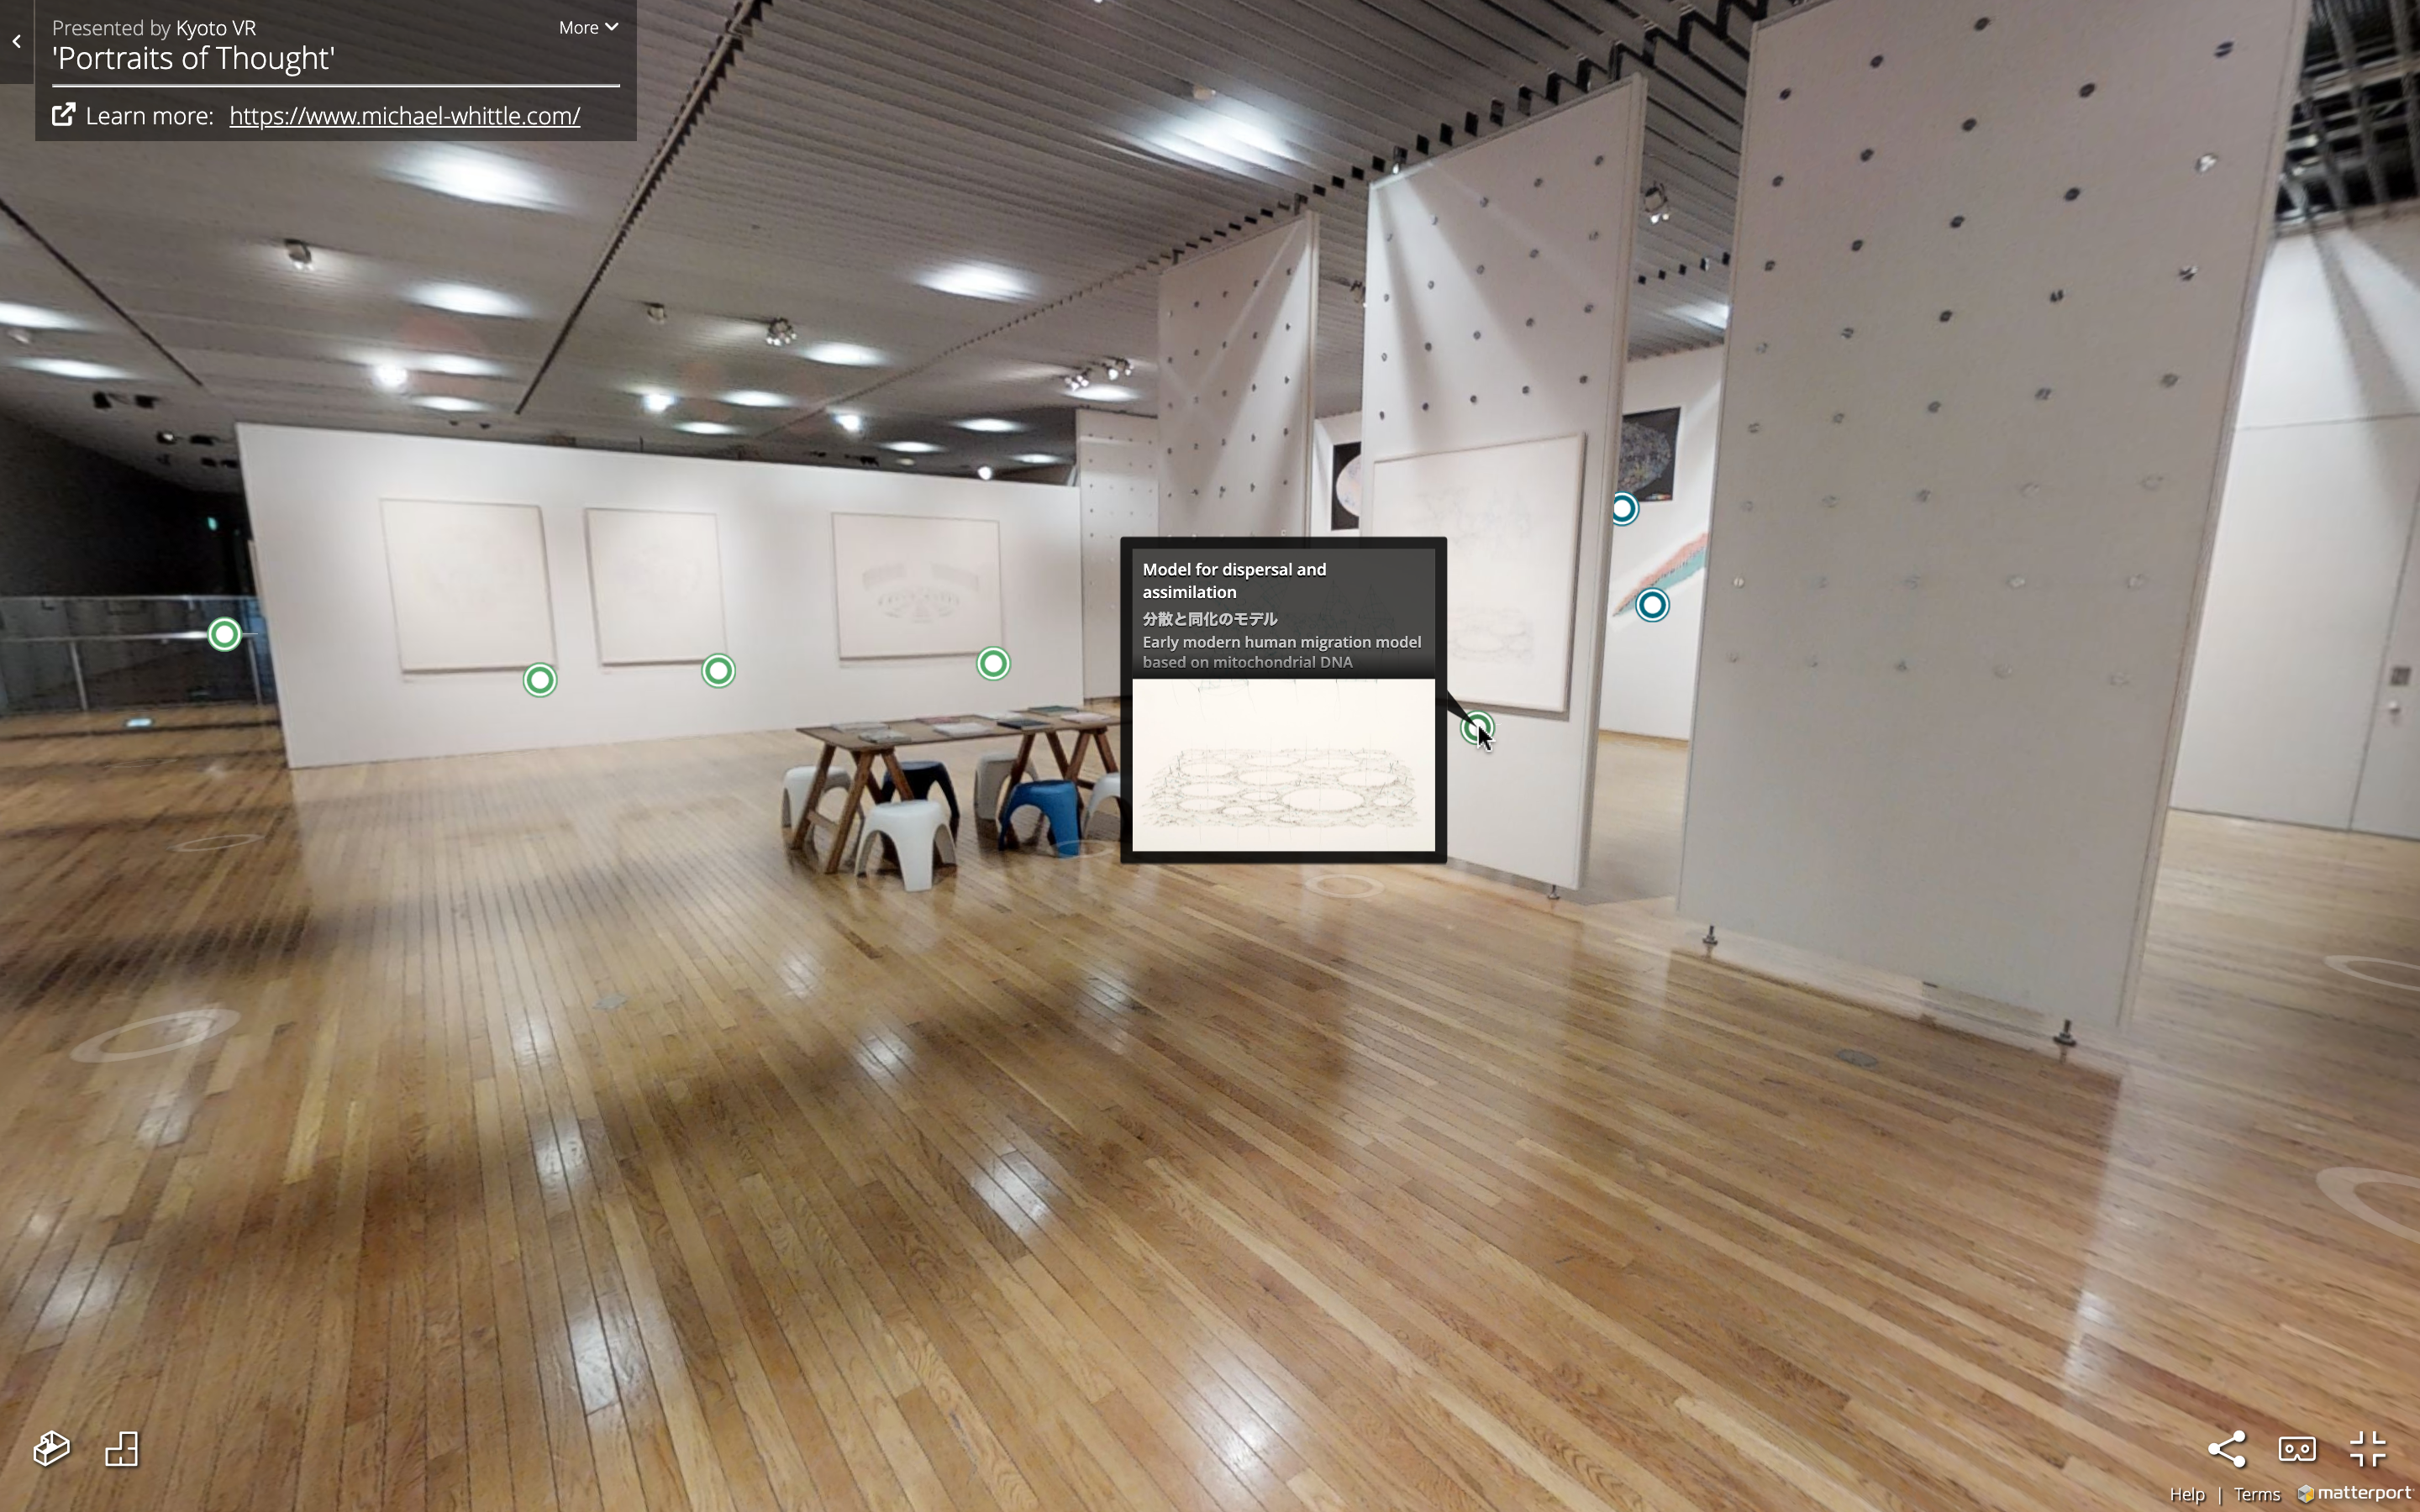
\includegraphics[width=.7\textwidth]{exhibition-scan.png}
    \caption{A screenshot of the 3D scan of `Portraits of Thought,' accessible
    from the web}
	\label{fig:exhibitionScan}
\end{figure}

\clearpage

\section{Conclusion and Future Work}
\label{sec:conclusionAndFutureWork}

Despite the numerous pivots this project went through, in the end we were able
to create a useful working prototype. The Editour is fully featured with
everything needed to build an audio tour anywhere in the world. ARuko allows
users to experience useful AR-enhanced tours in a pleasant and intuitive way.
Together they provide a complete platform for building augmented reality tour
guide apps.

Although the finished product works as intended, we encountered several issues
along the way. The changing scope and goal of the project meant we spent
several weeks researching and working on features that did not make it into the
final product (see Section~\ref{sec:alternativeArAppConcepts}), such as
displaying images in 3D AR space and playing spatialized audio. If we had
focused only on the features that made it into the final app from the start we
could have had more time to polish and refine those features.

Another challenge we faced was the difficulty in actually testing the app. The
Ritsumeikan University Biwako-Kusatsu campus we stayed at is about ninety
minutes away from Kinkaku-ji by expensive public transport, which meant that we
were only able to go to the site to test ARuko twice. We could test some basic
features from Ritsumeikan, but image recognition target existed only at
Kinkaku-ji. More extensive user testing at the actual site could have helped us
catch bugs earlier and lead to a more polished final product.

Despite these issues our team is happy with the product we delivered to Kyoto
VR. ARuko is not quite ready to be sold on app stores yet, but with a little
more development time it could easily be made ready. The UI could use more
testing with real users to make sure it is intuitive and easy to use. We also
intended to add a feature where the app could automatically download tour files
from the Editour server and import them without having to rebuild. We were not
able to complete this feature due to time constraints, but it could easily be
added because all of ARuko's business logic is abstracted and generalized to
support multiple tours. Editour also already supports requesting and downloading
the most recent versions of tours.

Editour is essentially feature complete. The most recent version, v1.3.0, can be
found in the GitHub repository
(\url{https://github.com/bandaloo/editour/releases/tag/v1.3.0}), and it contains
all the features necessary to create and edit tours. In the future Kyoto VR
should move it to a more powerful hosting provider (see
Section~\ref{sec:deployingTheEditourBackend}), but the current solution works
for now.

Given more time and resources, the app should be augmented to include a tour
browser that automatically downloads an unpacks tours from the Editour server.
More historic locations around Kyoto and Japan in general should be considered
for other tours. With the work our team has done Kyoto VR now has a complete
platform for creating and delivering unique tours, which can easily be expanded
upon in the future.

\clearpage % references should be on their own page

% references should be single spaced
\begin{singlespace}
	\printbibliography
	\addcontentsline{toc}{section}{References}
\end{singlespace}

\clearpage

\appendices
\section{Editour API Documentation}
\label{sec:editourAPIDocumentation}

Here is a list of API functions the Editour backend handles. The response is
usually a JSON like this with fields called \texttt{status} and \texttt{message}
The status is an HTTP status code like 200 (OK) or 404
(Not~Found)~\autocite{rfc7231}, and the message is a string or stringified JSON
that contains the data of the response.

\noindent\textbf{GET \texttt{/edit/:name}}

\begin{indented}{1cm}
	Returns the metadata file of the most recent tour with the given name. If
	successful, it returns a status of 200 and the stringified metadata as the
	message. If no tour with the given name is found it returns 404, and if the
	server encounters an internal error while processing the request it returns
	500.
\end{indented}

\noindent\textbf{GET \texttt{/tour/:name}}

\begin{indented}{1cm}
	This is the only API endpoint for which the response is not a JSON. Instead,
	the response is the zip file of the most recent version of the tour with the
	given name. Returns 404 if a tour with the given name isn't found or a 500
	if there is an internal server error while processing the request.
\end{indented}

\noindent\textbf{GET \texttt{/tours}}

\begin{indented}{1cm}
	Gets a list of unique tours on the server, returning a list of their names
	as the message of its response. Returns 200 if successful or 500 if there is
	an internal server error while processing the request.
\end{indented}

\noindent\textbf{POST \texttt{/edit}}

\begin{indented}{1cm}
	Used for editing an existing tour. This request should contain the fields
	\texttt{tourName}, \texttt{oldName}, and \texttt{metadata}, along with any
	number of files.  The server will use the new metadata as well as the old
	and new files to create a new version of an existing tour. Returns 201 if
	the tour was edited successfully, 400 if the request was invalid, 404 if the
	requested tour couldn't be found, or 500 if a server error occurred while
	processing the request.
\end{indented}

\noindent\textbf{POST \texttt{/upload}}

\begin{indented}{1cm}
	Used for uploading a new tour. This request should include a
	\texttt{tourName} field and a \texttt{metadata} field, along with any number
	of files. It verifies the uploaded tour and creates a zip for it on the
	server. Sends a 201 if the tour was created successfully, a 400 if the
	request is invalid, or a 500 if a server error is encountered.
\end{indented}

\noindent\textbf{DELETE \texttt{/tour/:name}}

\begin{indented}{1cm}
	Deletes all versions of the tour with the given name from the server.
	Returns 200 if successful, along with a message saying how many versions
	were deleted, 404 if no tour with that name could be found, or 500 if a
	server error was encountered.
\end{indented}

\clearpage

\section{Testing Survey Results}
\label{sec:testingSurveyResults}

After testing a near-complete prototype of ARuko at Kinkaku-ji on September
26\textsuperscript{th}, we had each test subject fill out a simple survey with
their thoughts on the app. The full results are listed below.

% for tabularx
% \newcolumntype{L}{>{\raggedright\arraybackslash\footnotesize}X}%

\begin{table}[h]
\begin{singlespace}
\begin{tabulary}{\textwidth}{ L | L | L | L | L | L }
	I enjoyed the audio tour & The image gallery added to the audio tour & I
	found the AR translation feature helpful & I found the AR map overlay
	helpful & The AR features were easy to use & Do you have any other thoughts
	on how to improve the experience? \\
	\hline

	Strongly agree & Agree & Strongly agree & Strongly agree & Agree & I thought
	the idea about a sound playing before the audio starts is a really good
	idea! \\

	Agree & Agree & Agree & Neutral & Neutral & Add a audio queue when a new
	track starts. Make the AR buttons bigger/easier to click. \\

	Agree & Agree & Strongly agree & Neutral & Agree & Increasing GPS accuracy
	of course. Adding a tracking "you are here" marker to the route. \\

	Strongly agree & Strongly agree & Strongly agree & Strongly agree & Strongly
	agree & Typo in the text on 4/11 towards the end \\

	Agree & Agree & Strongly agree & Disagree & Neutral & Zoom in ar mode \\
\end{tabulary}
\end{singlespace}
\caption{Results of final field test survey}
\label{tab:testingSurveyResults}
\end{table}

\end{document}

